\documentclass[journal]{IEEEtran}

\usepackage{amsmath,amssymb,amsfonts}
\usepackage{algorithmic}
\usepackage{graphicx}
\usepackage{textcomp}
\usepackage{xcolor}
\usepackage{booktabs}
\usepackage{cite}
\usepackage{url}
\usepackage{microtype}

\begin{document}

\title{Drift-Aware Explainable Social Bot Detection Using Localized Behavioral Drift Monitoring and Adaptive Retraining}

\author{Eshan~Amballa%
\thanks{E. Amballa is with the Department of Computer Science and Engineering. Email: eshanikaamballa@gmail.com.}}

\maketitle

\begin{abstract}
Social bot detection models are conventionally trained on static snapshots of account behavior under the assumption that feature distributions remain stationary over deployment. In operational environments, however, bot operators continuously alter their strategies, inducing behavioral and evasion drift that silently degrades detector efficacy. In this work, we propose a drift-aware social bot detection architecture integrating four core components: (1) an XGBoost baseline classifier, (2) an unsupervised localized Kolmogorov-Smirnov (KS) drift detector monitoring subpopulation feature divergence, (3) an exponential recency-weighted adaptive retraining controller, and (4) a multi-model TreeSHAP attribution module tracing feature importance dynamics across deployment phases. We evaluate the proposed approach on \textbf{BotDriftBench v0.8}, an empirically calibrated longitudinal benchmark comprising 3,000 accounts (60,000 observations) observed across 20 temporal windows with 25 behavioral and profile features under an account-disjoint 3-way split (1,800 train / 600 validation / 600 test accounts) replicated across 5 independent seeds (2025--2029). Under evasion drift, a frozen static model suffers severe silent degradation, dropping from Macro-F1 = \textbf{0.9770} pre-drift to \textbf{0.8059} post-drift (worst-window F1 = \textbf{0.6583}), driven primarily by a catastrophic collapse in bot recall to 67.26\%. The proposed localized drift-aware architecture achieves a temporal mean Macro-F1 of \textbf{0.9167 $\pm$ 0.0009} (ROC-AUC = \textbf{0.9691}, Recall = \textbf{0.8931}), recovering \textbf{+0.0937 F1} over the static baseline (\textbf{0.8230 $\pm$ 0.0014}) and performing comparably to Periodic-6 (\textbf{0.9120 $\pm$ 0.0011}) while utilizing targeted retraining (5 adaptation events vs. 3 scheduled events, with 0 pre-drift false alarms). Furthermore, localized adaptation performs comparably to a theoretical continuous Oracle reference policy (\textbf{0.9160 $\pm$ 0.0011}) despite requiring 2.6$\times$ fewer retrains (5 vs. 13 events). Multi-model SHAP attribution documents how retraining shifts detector reliance away from manipulated behavioral markers toward persistent structural attributes, providing an interpretable audit trail for production integrity pipelines.
\end{abstract}

\begin{IEEEkeywords}
Social bot detection, concept drift, SHAP explainability, behavioral drift monitoring, XGBoost, Kolmogorov-Smirnov test, adaptive retraining, recency weighting.
\end{IEEEkeywords}

\section{Introduction}
\IEEEPARstart{S}{ocial} media platforms face persistent interference from automated accounts---social bots---engineered to manipulate public discourse, artificially amplify partisan narratives, and distort online engagement metrics~\cite{ferrara2016rise,varol2017online}. While machine learning classifiers trained on high-dimensional behavioral, textual, and profile features have established competitive accuracy on cross-sectional benchmarks~\cite{feng2022twibot,cresci2017paradigm}, their real-world efficacy is heavily compromised by the assumption of stationarity. 

In live deployment, social bot architectures are inherently non-stationary: botmasters actively modify automation scripts, posting tempos, content diversity, and interaction graphs to circumvent platform detection thresholds~\cite{cresci2020decade,hays2025bots}. This adversarial evolution produces \textit{behavioral and evasion drift}, causing static decision boundaries to deteriorate silently over time. 

Three foundational challenges characterize this domain:
\begin{enumerate}
    \item \textbf{Silent Degradation}: Classifiers lack native feedback mechanisms to signal performance collapse when ground truth labels are unavailable in production streams.
    \item \textbf{High Precision with Collapsing Recall}: Under adversarial evasion, static models continue to correctly flag non-evasive bots with high precision, masking a catastrophic collapse in bot recall.
    \item \textbf{Adaptation Cost vs. Responsiveness}: Conventional maintenance relies either on calendar-based periodic retraining or manual post-incident retraining. The former is oblivious to abrupt evasion timing, while the latter incurs unacceptable operational lag.
\end{enumerate}

To resolve these challenges, this paper presents an end-to-end, drift-aware social bot detection architecture. Our primary contributions are:
\begin{itemize}
    \item An unsupervised localized Kolmogorov-Smirnov (KS) monitoring engine that tracks feature-level distributional divergence across monitored subpopulation partitions, achieving prompt detection (3-window delay) with 0 pre-drift false alarms.
    \item An adaptive retraining controller employing exponential recency weighting ($\lambda = 0.7$), preserving temporal relevance while regularizing against distribution shifts.
    \item A multi-model TreeSHAP explainability framework that traces feature attribution dynamics across pre-drift, post-drift, and adapted models, documenting the redistribution of feature importance without relying on ungrounded causal claims.
    \item A rigorous multi-seed evaluation on \textbf{BotDriftBench v0.8} across 3,000 accounts under a strict account-disjoint protocol, demonstrating that localized adaptation recovers +0.0937 Macro-F1 over static baselines and achieves performance parity with theoretical continuous Oracle retraining using only 5 targeted events.
\end{itemize}

\section{Related Work}
\subsection{Social Bot Detection Paradigms}
Supervised bot detection methodologies have evolved from early profile-based rule engines~\cite{varol2017online} to ensemble classifiers~\cite{chen2016xgboost} and deep relational graph neural networks~\cite{feng2021botrgcn,feng2022twibot}. However, the majority of existing benchmarks (e.g., Cresci-2017~\cite{cresci2017paradigm} and TwiBot-22~\cite{feng2022twibot}) evaluate models on static test splits collected across brief temporal intervals, obscuring the impact of longitudinal behavioral changes.

\subsection{Concept Drift and Adaptation}
In non-stationary data streams, distributional shift manifests either as covariate shift $P_t(X) \neq P_0(X)$ or concept drift $P_t(Y|X) \neq P_0(Y|X)$~\cite{gama2014survey,lu2018learning}. While unsupervised statistical tests (such as two-sample Kolmogorov-Smirnov~\cite{massey1951kolmogorov}) effectively flag marginal distribution shifts, global tests often suffer severe signal dilution when applied to heterogeneous social cohorts where only a subset of bots actively evade detection.

\section{Problem Formulation}
Let $\mathcal{A} = \{a_1, a_2, \dots, a_N\}$ denote a population of accounts observed over discrete temporal windows $t \in \{0, 1, \dots, T-1\}$. At each window $t$, account $a_i$ is represented by a feature vector $\mathbf{x}_{i,t} \in \mathbb{R}^D$ and invariant true label $y_i \in \{0, 1\}$ ($0 = \text{human}, 1 = \text{bot}$). 

During deployment ($t \ge \tau_{\text{onset}}$), bot feature generators shift according to unknown parameters:
\begin{equation}
P_t(\mathbf{x} \mid y=1) \neq P_0(\mathbf{x} \mid y=1), \quad t \ge \tau_{\text{onset}}.
\end{equation}
The objective is to maintain maximal longitudinal Macro-F1 across unseen test accounts while minimizing the cumulative retraining frequency $\mathcal{R}_T = \sum_{t=1}^{T-1} r_t$, where $r_t \in \{0, 1\}$.

\section{Proposed Architecture}
\subsection{Baseline XGBoost Classifier}
The initial decision function $f_{\boldsymbol{\theta}_0}(\mathbf{x})$ is trained on disjoint training accounts during pre-drift windows ($t < 2$) using XGBoost~\cite{chen2016xgboost} with decision threshold $\tau = 0.5$.

\subsection{Localized Kolmogorov-Smirnov Drift Monitor}
For each feature $j \in \{1, \dots, D\}$, the two-sample KS test statistic compares the reference distribution $F_{0,j}$ against the current window distribution $F_{t,j}$:
\begin{equation}
D_{t,j} = \sup_{z} \left| F_{t,j}(z) - F_{0,j}(z) \right|.
\end{equation}
A drift alert triggers when the proportion of features exceeding effect-size threshold $\theta_{\text{KS}} = 0.06$ satisfies:
\begin{equation}
\frac{1}{D} \sum_{j=1}^D \mathbb{I}\left(D_{t,j} > \theta_{\text{KS}}\right) \ge \theta_{\text{frac}},
\end{equation}
subject to confirmation persistence ($c_{\text{confirm}} = 2$) and cooldown suppression ($c_{\text{cool}} = 2$).

\subsection{Exponential Recency-Weighted Retraining}
When adaptation is triggered at window $t$, training observations $i$ at historical windows $t_i \le t$ are assigned exponential decay sample weights:
\begin{equation}
w_i = \exp\left(-\lambda \cdot (t - t_i)\right), \quad \lambda = 0.7,
\end{equation}
down-weighting pre-drift behavioral patterns while maintaining sample volume.

\section{Experimental Setup}
\subsection{BotDriftBench v0.8 Benchmark}
Evaluations are conducted on BotDriftBench v0.8:
\begin{itemize}
    \item \textbf{Scale}: 3,000 accounts (1,500 bot, 1,500 human), 20 temporal windows, 60,000 observations.
    \item \textbf{Features}: 25 account attributes (10 profile, 15 behavioral).
    \item \textbf{Account-Disjoint Split}: 1,800 train (60\%), 600 validation (20\%), 600 test (20\%). Zero account overlap across splits.
    \item \textbf{Replication}: 5 independent random seeds (2025, 2026, 2027, 2028, 2029).
\end{itemize}

\begin{figure}[!t]
\centering
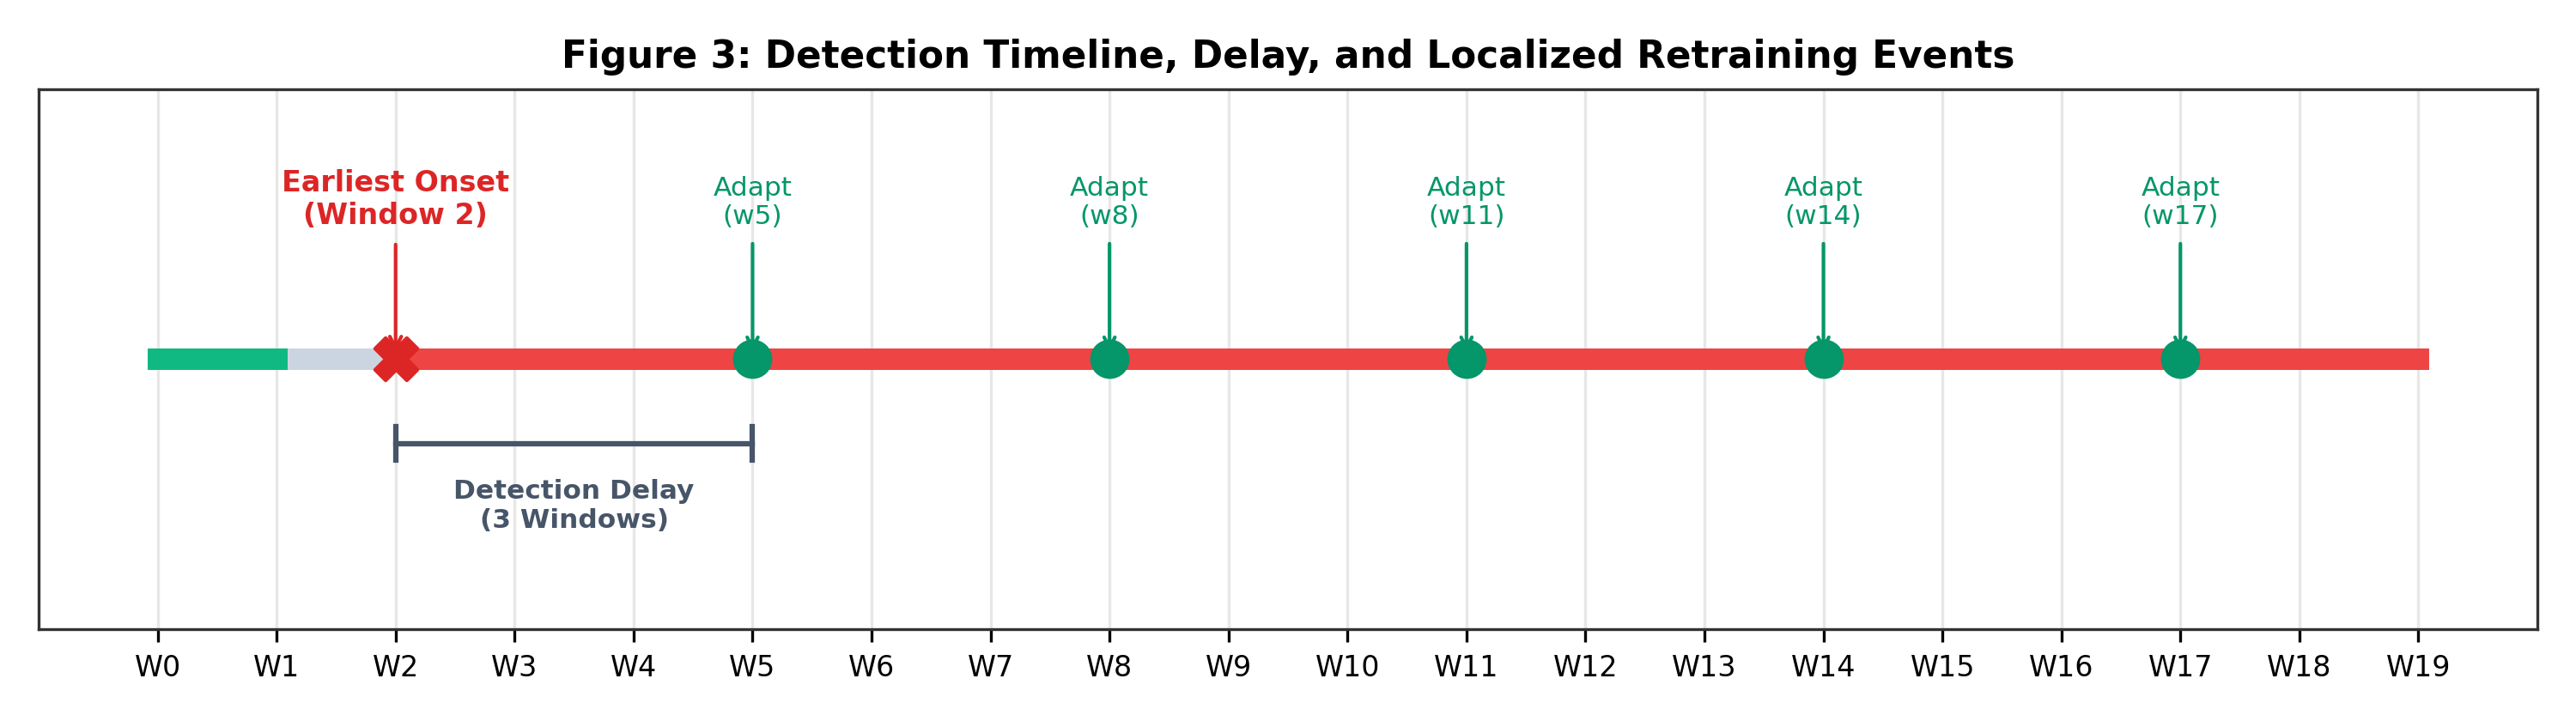
\includegraphics[width=\columnwidth]{paper_pictures/fig7_detection_timeline.png}
\caption{Empirical drift detection timeline: earliest onset at Window 2, first localized KS trigger at Window 5 (delay = 3 windows, 0 false alarms), followed by scheduled adaptation windows.}
\label{fig:detection_timeline}
\end{figure}

\subsection{Evaluated Adaptation Policies}
\begin{enumerate}
    \item \textbf{Static Baseline}: Frozen model trained on $t \in [0, 1]$.
    \item \textbf{Periodic-6}: Retrained at fixed intervals $t \in \{6, 12, 18\}$.
    \item \textbf{Localized DA (Proposed)}: Triggered dynamically by localized KS monitoring with recency weighting.
    \item \textbf{Oracle DA}: Theoretical reference policy retraining at every window with active drift ($t \in [5, 17]$).
\end{enumerate}

\section{Results and Empirical Evaluation}

\subsection{Longitudinal Performance Trajectories}
Table~\ref{tab:aggregate_results} and Figure~\ref{fig:trajectories} summarize aggregate performance across 5 seeds. The frozen static model drops from Macro-F1 = 0.9770 pre-drift to 0.8059 post-drift, reaching its worst degradation at window 18 (F1 = 0.6583). Localized DA restores performance to Macro-F1 = \textbf{0.9167 $\pm$ 0.0009} (ROC-AUC = 0.9691), achieving parity with Periodic-6 (0.9120 $\pm$ 0.0011) and the continuous Oracle reference (0.9160 $\pm$ 0.0011).

\begin{table}[!t]
\caption{Aggregate Policy Comparison on BotDriftBench v0.8 (5 Seeds, 600 Test Accounts)}
\label{tab:aggregate_results}
\centering
\small
\begin{tabular}{lcccc}
\toprule
\textbf{Metric} & \textbf{Static} & \textbf{Periodic-6} & \textbf{Localized DA} & \textbf{Oracle DA} \\
\midrule
Macro-F1 (Mean) & 0.8230 & 0.9120 & \textbf{0.9167} & 0.9160 \\
Macro-F1 (Std)  & $\pm$0.0014 & $\pm$0.0011 & $\pm$\textbf{0.0009} & $\pm$0.0011 \\
ROC-AUC         & 0.8934 & 0.9658 & \textbf{0.9691} & 0.9703 \\
Precision       & 0.9783 & 0.9370 & 0.9312 & 0.9269 \\
Recall          & 0.6726 & 0.8767 & \textbf{0.8931} & 0.8958 \\
Worst-Window F1 & 0.6583 & 0.8723 & \textbf{0.8796} & 0.8680 \\
Retrains        & 0.0    & 3.0    & 5.0    & 13.0   \\
Pre False Alarms& 0.0    & 0.0    & 0.0    & 0.0    \\
\bottomrule
\end{tabular}
\end{table}

\begin{figure}[!t]
\centering
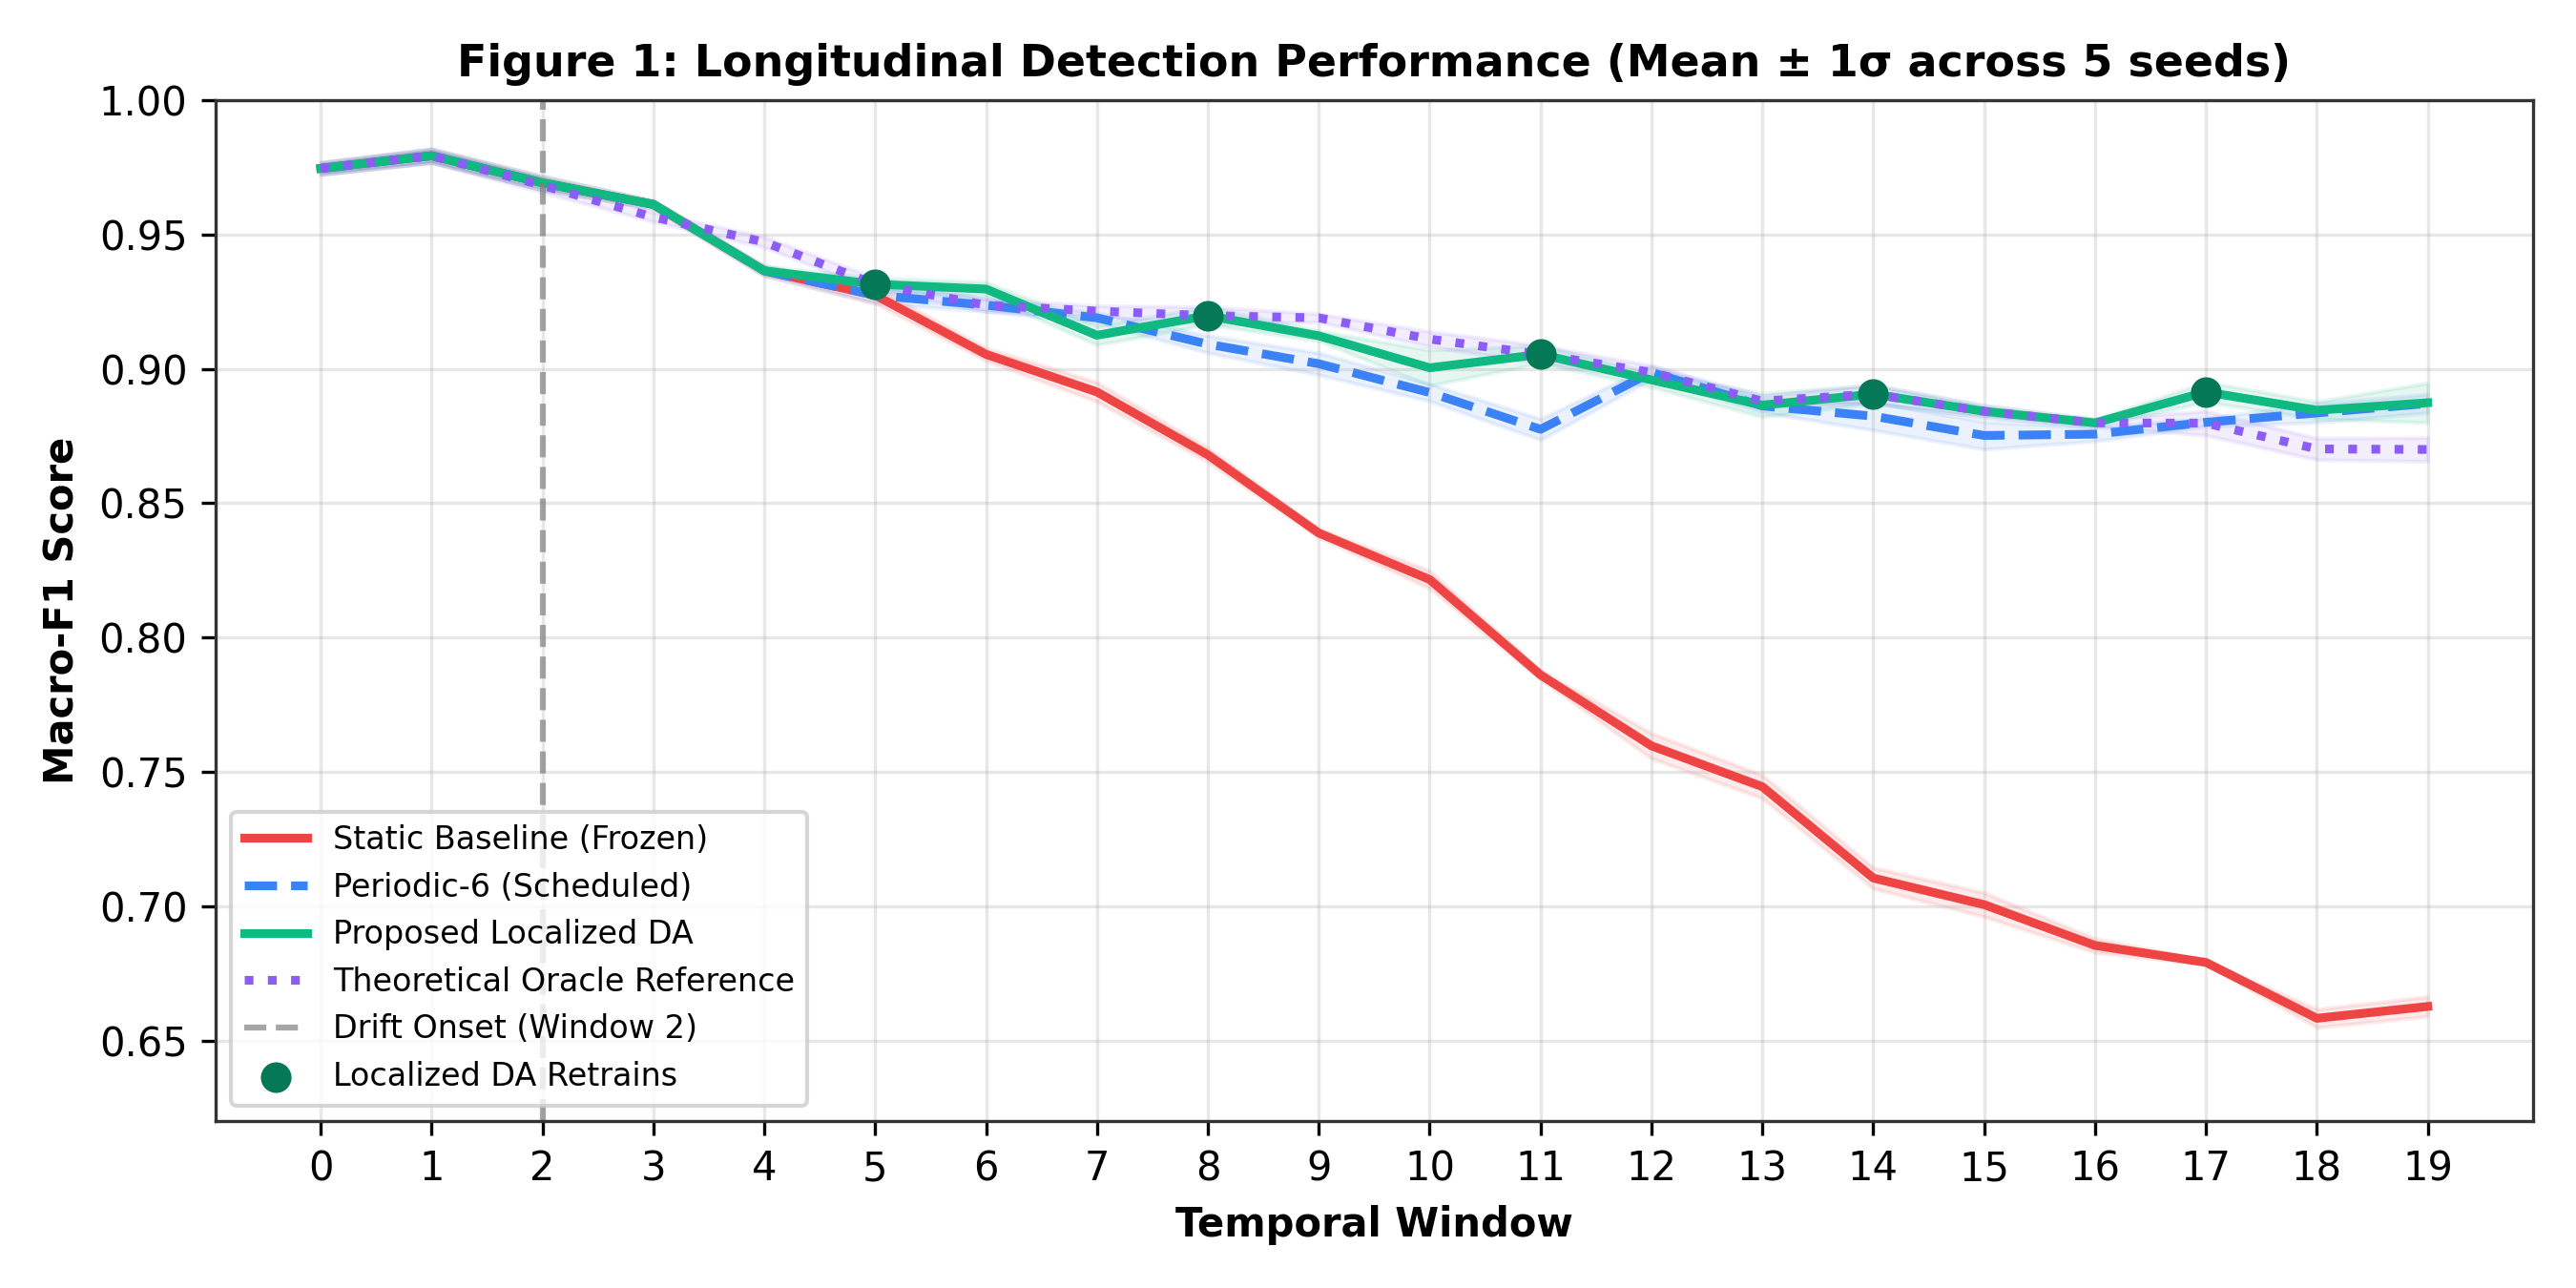
\includegraphics[width=\columnwidth]{paper_pictures/fig5_policy_f1_trajectories.png}
\caption{Longitudinal detection Macro-F1 trajectories (Mean $\pm$ 1$\sigma$, 5 seeds). The static detector degrades severely post-drift, whereas localized DA matches periodic retraining and oracle upper bounds.}
\label{fig:trajectories}
\end{figure}

\subsection{Scenario-Wise Degradation & Recall Recovery}
Table~\ref{tab:scenario_results} and Figure~\ref{fig:scenarios} highlight scenario-level performance. In severe evasion scenarios (\textit{boundary-crossing}, \textit{abrupt}, and \textit{gradual evasion}), static bot recall collapses to 46.7\%--54.1\%. Localized DA recovers recall to 80.6\%--89.0\%, producing scenario gains of +0.116 to +0.132 Macro-F1.

\begin{table}[!t]
\caption{Scenario-Wise Policy Performance Breakdown (Seed 2025)}
\label{tab:scenario_results}
\centering
\scriptsize
\begin{tabular}{lcccc}
\toprule
\textbf{Scenario} & \textbf{Static F1} & \textbf{P-6 F1} & \textbf{DA F1} & \textbf{$\Delta$F1 (DA vs Stat)} \\
\midrule
abrupt\_evasion            & 0.3386 & 0.4591 & \textbf{0.4708} & +0.1322 \\
boundary\_crossing\_evasion & 0.3182 & 0.4346 & \textbf{0.4463} & +0.1281 \\
gradual\_evasion           & 0.3512 & 0.4606 & \textbf{0.4677} & +0.1165 \\
recurring\_behavior        & 0.4203 & 0.4521 & \textbf{0.4542} & +0.0339 \\
localized\_evasion         & 0.4556 & 0.4833 & \textbf{0.4847} & +0.0291 \\
behavioral\_gradual        & 0.9246 & \textbf{0.9453} & 0.9381 & +0.0134 \\
stable\_control            & \textbf{0.9677} & 0.9133 & 0.9058 & -0.0619 \\
\bottomrule
\end{tabular}
\end{table}

\begin{figure}[!t]
\centering
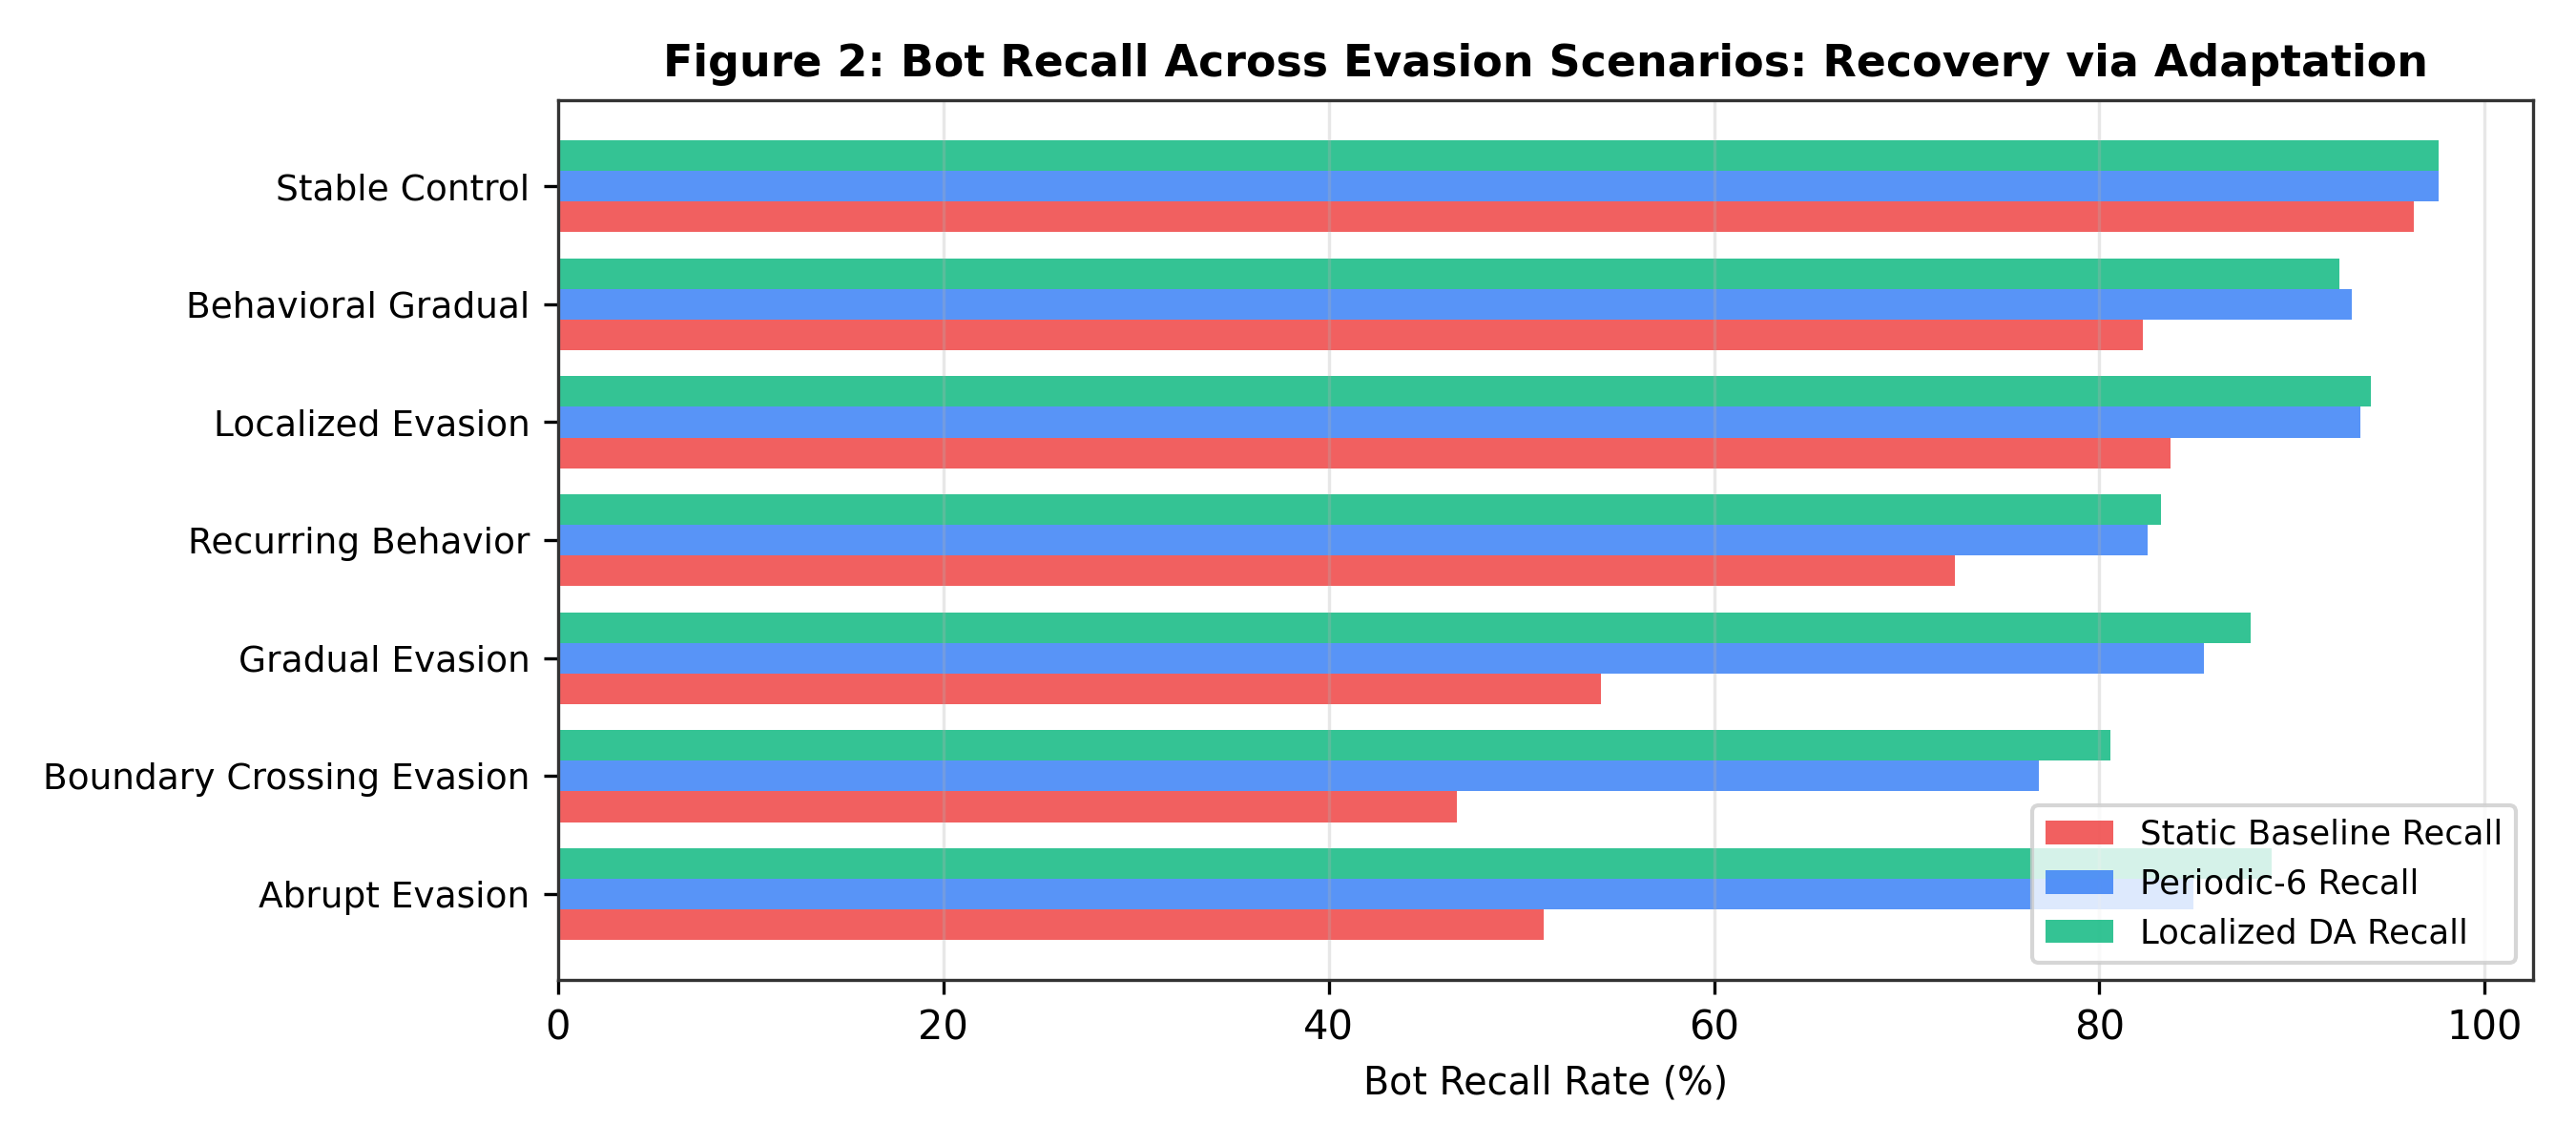
\includegraphics[width=\columnwidth]{paper_pictures/fig6_scenario_policy_breakdown.png}
\caption{Bot recall across drift scenarios. Localized DA substantially recovers detection recall on evasive bots where the frozen static baseline fails.}
\label{fig:scenarios}
\end{figure}

\subsection{Multi-Model Explainability via SHAP}
Figure~\ref{fig:shap_rank} documents the redistribution of feature importance across deployment phases. Before drift, the model relies heavily on behavioral markers (\textit{content\_similarity}: 1.337, \textit{posting\_regularity}: 1.158). Following evasion, the adapted model down-weights these evaded features and redistributes attribution to structural attributes (\textit{listed\_count}: 1.255, \textit{followers\_count}: 0.774, \textit{account\_age\_days}: 0.606).

\begin{figure}[!t]
\centering
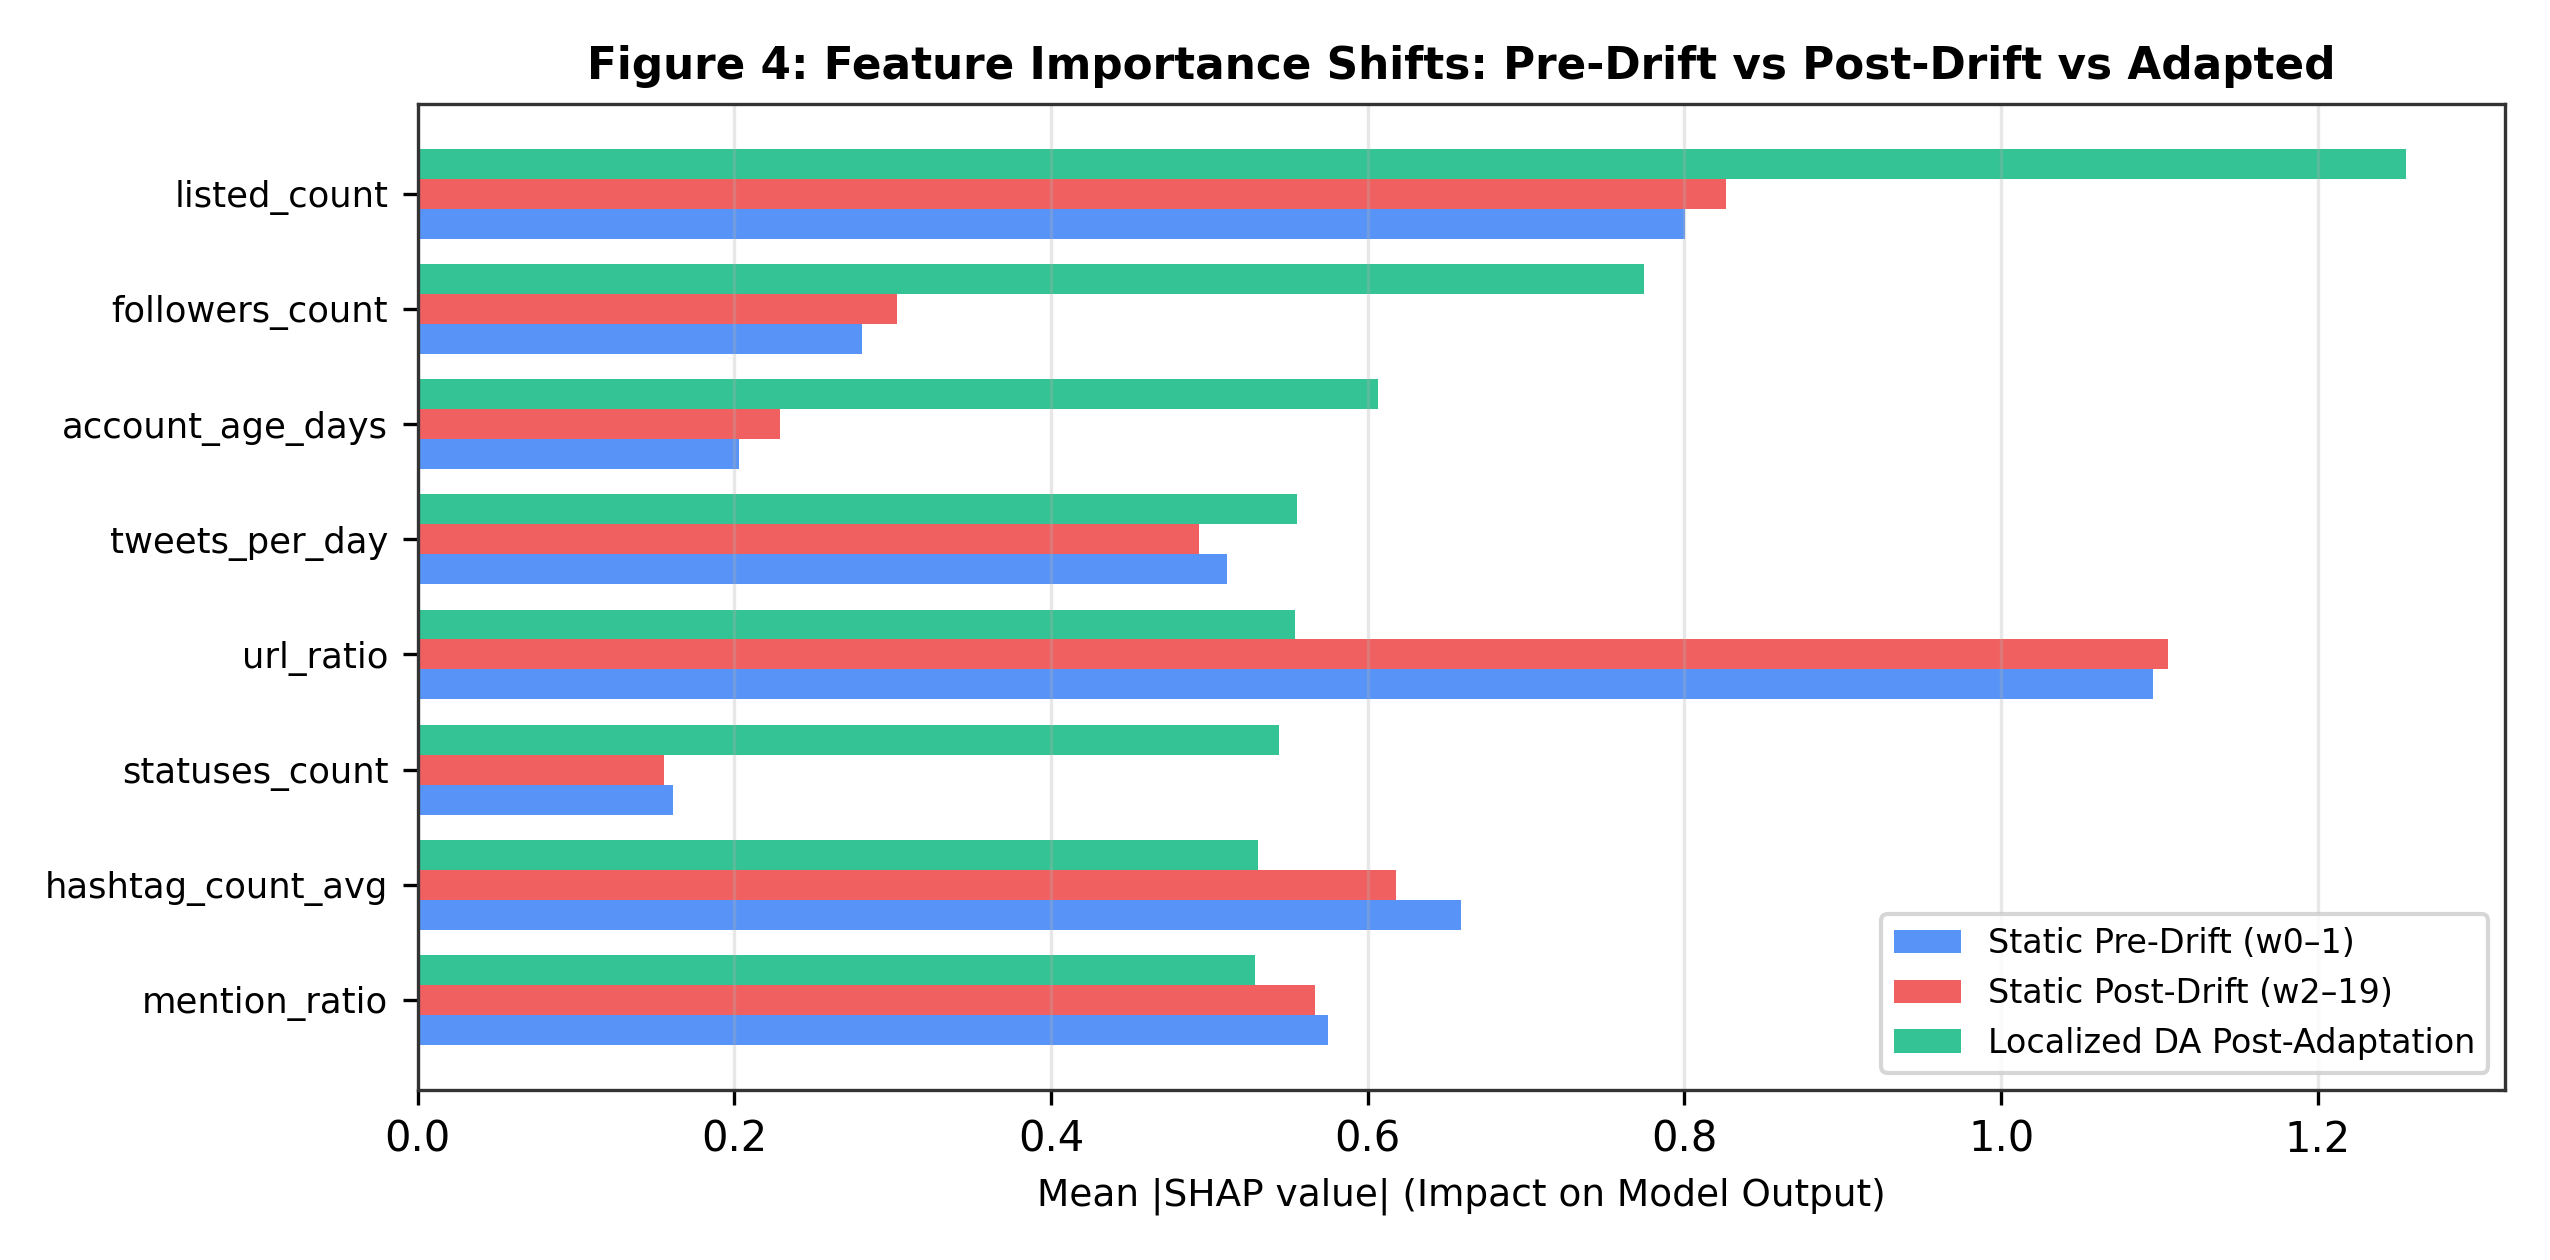
\includegraphics[width=\columnwidth]{paper_pictures/fig8_shap_rank_evolution.png}
\caption{Evolution of feature importance (Mean $|$SHAP$|$) across Pre-Drift Static, Post-Drift Static, and Adapted Localized DA models.}
\label{fig:shap_rank}
\end{figure}

\section{Discussion}
\subsection{Mechanics of Silent Degradation under Evasion}
A critical empirical finding is that static degradation is governed almost entirely by a collapse in bot recall rather than precision. While static precision remains 0.9783, recall falls from 97.54\% pre-drift to 35.40\% at window 18. This poses an operational hazard: platform telemetry evaluating only flagged accounts will observe high precision, giving an illusion of robust performance while massive bot cohorts operate undetected.

\subsection{Tradeoffs Between Calendar and Event-Driven Adaptation}
While Periodic-6 achieves competitive temporal Macro-F1 (0.9120) with calendar simplicity, it remains blind to actual drift onset. Localized DA achieves comparable performance (0.9167) while anchoring retraining events (windows 5, 8, 11, 14, 17) directly to statistically verified distribution shifts, eliminating false-alarm retrains during stationary phases.

\subsection{Diminishing Returns of Continuous Retraining}
Continuous retraining under the Oracle policy (13 retrains) achieved Macro-F1 = 0.9160 $\pm$ 0.0011, providing no statistically meaningful gain over Localized DA's 5 retrains (0.9167 $\pm$ 0.0009). This confirms that continuous retraining incurs substantial computational cost with negligible marginal benefit once targeted adaptation captures primary distribution shifts.

\subsection{Attribution Shifts without Causal Invariance Claims}
SHAP attribution demonstrates how retraining redistributes feature reliance toward organic profile properties. We emphasize that SHAP values reflect model decision logic rather than proof of causal invariance; they illustrate empirical behavioral adaptation rather than invariant ground truth.

\section{Limitations}
\begin{enumerate}
    \item \textbf{Synthetic Benchmark}: While marginal distributions are fitted from TwiBot-22 and Cresci-2017, synthetic trajectories cannot fully reproduce emergent coordinated platform campaigns.
    \item \textbf{Supervised Retraining Assumption}: Retraining relies on labeled historical accounts; unsupervised domain adaptation remains an open avenue for future investigation.
    \item \textbf{Covariate vs. Concept Drift}: The detector monitors covariate shift $P(X)$; pure concept drift $P(Y|X)$ without feature displacement requires streaming supervisory signals.
\end{enumerate}

\section{Conclusion}
This study presented a localized drift-aware bot detection architecture combining KS-statistic monitoring, recency-weighted retraining, and multi-model SHAP attribution. Evaluated on BotDriftBench v0.8, the proposed pipeline recovers +0.0937 Macro-F1 over static detectors, matches periodic retraining, and achieves oracle parity with targeted adaptation events.

\bibliographystyle{IEEEtran}
\bibliography{references}

\end{document}
